\chapter{Temperature and Ideal Gases}
\begin{itemize}
    \item From empirical results, we know that there appears to be a \emph{linear} trend, wherein pressure and volume decrease, when temperature decreases. So, there must be a temperature where pressure is zero, and a temperature where volume is zero. Empirical data shows that the temperature at which this occurs is the same for all gases under all experimental conditions. This temperature is known as \emph{absolute zero}.
    \item The \emph{Zeroth Law of Thermodynamics} states that if bodies \(A\) and \(B\) are separately in thermal equilibrium with body \(C\), then bodies \(A\) and \(B\) are in thermal equilibrium with each other.
    \item \emph{One mole} is defined as the amount of substance that contains as many elementary particles as there are atoms in 0.012kg of carbon-12.
    \item \emph{Avogadro's Constant \(N_A\)} is the number of atoms in 0.012kg of carbon-12.
    \item Celsius-Kelvin conversion: \(T\ {^\circ}\text{C}=(T+273.15)\ \text{K}\). 
    \begin{figure}[H]
        \centering
        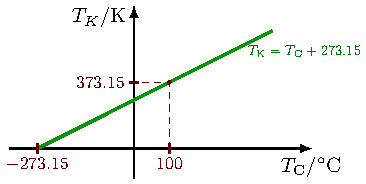
\includegraphics{../images/Celcius-Kelvin/Celcius-Kelvin.pdf}
        \caption{\ref{source:celsius-kelvin} Kelvin against celsius graph.}
        \label{fig:celsius-kelvin}
    \end{figure}
    \item An \emph{ideal gas} is a \emph{hypothetical gas} that \emph{perfectly} obeys the \emph{equation of state} for an ideal gas, at \emph{all} pressures, temperatures, and volumes. The equation of state is \(pV=nRT\), where 
    \begin{enumerate}
        \item[\(p:\)] pressure of ideal gas
        \item[\(V:\)] volume of ideal gas
        \item[\(n:\)] number of moles of ideal gas
        \item[\(R:\)] molar gas constant
        \item[\(T:\)] temperature of ideal gas.     
    \end{enumerate}
    \item There is no ideal gas in nature, but at \emph{low pressures} and \emph{high temperatures}, real gases behave like ideal gases.
    \item \emph{Boyle's Law}. When the temperature of an ideal gas remains constant, the product of its pressure \(p\) and volume \(V\) is constant. i.e. \(p_1V_1=p_2V_2\).
    \item \emph{Charles' Law}. When the pressure of an ideal gas remains constant, its volume \(V\) is directly proportional to its thermodynamic temperature \(T/K\). i.e. \(V_1/T_1=V_2/T_2\).
    \item \emph{Gay-Lussac's Law}. When the volume of an ideal gas remains constant, its pressure \(p\) is directly proportional to its thermodynamic temperature \(T/K\). i.e. \(p_1/T_1=p_2/T_2\).
    \item Let \(n\) be the amount of gas in moles and the integer \(N\) be the number of gas molecules. Then, for the molar gas constant \(R=8.31\) J K\(^{-1}\) mol\(^{-1}\) and Boltzmann's constant \(k=1.38\cdot 10^{-23}\) J K\(^{-1}\), the equation of state for an ideal gas is \(pV=nRT=NkT\).
    \item Some useful conversions. For \(\ce{_Z^A\text{X}}\), we have the ratio \(1\text{ mole}:Z\text{ grams}\) and \(n=\frac{N}{N_A}=\frac{m/g}{Z}\).
    % E.g. \(\ce{^{12}_6\text{C}}\) and \(\ce{^{16}_8\text{O}}\) so the molecular mass of CO is \(12+16=28\) g/mol.
    \newpage
    \item ~\\[-3mm]
    \begin{tabular}{|Sc|Sl|}
        \hline
        & Assumptions of the Kinetic Theory of Gases\\
        \hline
        \textbf{M} & 
        \begin{tabular}{@{}Sl@{}}
            The molecules of the gas are in \emph{rapid} and \emph{random} motion.
          \end{tabular}\\
        \hline
        \textbf{A} & 
        \begin{tabular}{@{}Sl@{}}
            There are \emph{no intermolecular} attractive forces.
        \end{tabular}\\
        \hline
        \textbf{N} & 
        \begin{tabular}{@{}Sl@{}}
        Any gas consists of a \emph{very large number} of molecules.
        \end{tabular}\\
        \hline
        \textbf{T} & 
        \begin{tabular}{@{}Sl@{}}
        The duration of collisions is negligible compared\\ to the time interval between collisions.
        \end{tabular}\\
        \hline
        \textbf{E} & 
        \begin{tabular}{@{}Sl@{}}
        The collisions between gas molecules, and between\\ gas molecules and the container walls are \emph{perfectly elastic}.
        \end{tabular}\\
        \hline
        \textbf{V} & 
        \begin{tabular}{@{}Sl@{}}
        The volume of the gas molecules themselves is negligible \\compared to the volume of the container.
        \end{tabular}\\
        \hline
    \end{tabular}
    \item How would the force exerted by gas differ in the presence of intermolecular forces, compared to the ideal case? Particles would attract each other, so the average force on the wall will decrease.   
    \item Real gases are approximately ideal at high temperatures and low pressures.
    \item Deriving \(p=\frac{1}{3}\frac{Nm}{V}\langle c^2 \rangle\) for an ideal gas:
    \begin{enumerate}
        \item Consider a cubic container of side \(l\) containing \(N\) molecules, each of mass m.
        \item The change in momentum of one molecule due to its \emph{elastic} collision with the container wall is \(2mc_x\)
        \item The time interval between collisions of this molecule with the same wall is \(\Delta t=\frac{2l}{c_x}\).
        \item By Newton's 2nd Law, the net force \(F\) experienced by one molecule is equal to the rate of change of momentum it experiences. i.e. \(F=\frac{2mc_x}{\frac{2l}{c_x}}=\frac{mc_x^2}{l}\).
        \item By Newton's 3rd Law, since the molecule and the container wall form an action-reaction pair, the net force experienced by the container wall (due to this one molecule) is \(F\).
        \item The pressure experienced by the wall due to this one molecule is \(p=\frac{mc_x^2}{l^3}=\frac{mc_x^2}{V}\).
        \item The pressure experienced by the wall due to \(N\) molecules is \(p_N=\frac{Nmc_x^2}{V}\).
        \item The molecules can move in three directions, so \(c^2=c_x^2+c_y^2+c_z^2\). Since the molecules' motion is random, \(\langle c_x^2 \rangle=\langle c_y^2 \rangle=\langle c_z^2 \rangle\). Hence \(\langle c^2 \rangle=3\langle c_x^2 \rangle\). 
        \item Now, \(p_N=\frac{Nm\langle \frac{1}{3}c^2\rangle}{V}=\frac{1}{3}\frac{Nm\langle c^2 \rangle}{V}\).
    \end{enumerate}
    \item The mean translational kinetic energy of an ideal gas molecule molecule is \(\frac{1}{2}m \langle c^2 \rangle=\frac{3}{2}kT\).
    \item The total translational kinetic energy of \(N\) ideal gas molecules is \(\frac{3}{2}NkT=\frac{3}{2}nRT=\frac{3}{2}pV\). 
\end{itemize}